
\documentclass{jtetiproposalskripsi}

%-----------------------------------------------------------------
%Disini awal masukan untuk data proposal skripsi
%-----------------------------------------------------------------
\titleind{APLIKASI OBJEK WISATA KABUPATEN JEMBER BERBASIS ANDROID}
\fullname{Lola Yunita Audiana}

\idnum{1200631042}

\approvaldate{13 Januari 2015}

\degree{Sarjana Komputer}

\yearsubmit{2015}

\program{Manajemen Informatika}

\headprogram{Sarjiya, S.T., M.T., Ph.D.}

\dept{}

\firstsupervisor{Sigit Basuki Wibowo, S.T., M.Eng.}
\firstnip{1976 0501 2002 12 1 002}

\secondsupervisor{Bimo Sunarfri Hantono, S.T., M.Eng.}
\secondnip{1977 0131 2002 12 1 003}


%-----------------------------------------------------------------
%Disini akhir masukan untuk data proposal skripsi
%-----------------------------------------------------------------

\begin{document}

\cover

\approvalpage

%-----------------------------------------------------------------
%Disini akhir masukan untuk muka skripsi
%-----------------------------------------------------------------

%-----------------------------------------------------------------
%Disini awal masukan Intisari
%-----------------------------------------------------------------
\begin{abstractind}
Jember merupakan kabupaten yang mempunyai potensi pariwisata yang banyak dikunjungi wisatawan. Salah satu informasi penting dalam bidang pariwisata yaitu adanya Aplikasi wisata yang mudah diaplikasikan dimana saja dan kapan saja. Untuk memudahkan itu para masyarakat khususnya wisatawan dibutuhkan aplikasi objek wisata yang dikemas dalam bentuk multimedia yang dapat diaplikasikan di handphone (mobile) sehingga lebih terjangkau. Menggunakan Eclips, aplikasi yang dibuat berupa aplikasi objek wisata kabupaten Jember yang bertujuan memudahkan para wisatawan dalam mendapatkan informasi mengenai lokasi objek pariwisata yang ada di kota Jember. Aplikasi objek wisata Kabupaten Jember berbasis android ini dapat dijadikan pedoman bagi para pengguna atau wisatawan yang akan berkunjung ke Kabupaten Jember. 


\bigskip
\textbf{Kata kunci} : Aplikasi objek wisata Kabupaten Jember, Eclips,Handphone.
\end{abstractind}
%-----------------------------------------------------------------
%Disini akhir masukan Intisari
%-----------------------------------------------------------------

\tableofcontents
\addcontentsline{toc}{chapter}{DAFTAR ISI}
\selectlanguage{bahasa}\clearpage\pagenumbering{arabic}\setcounter{page}{1}

%-----------------------------------------------------------------
%Disini awal masukan untuk Bab
%-----------------------------------------------------------------
\chapter{LATAR BELAKANG}

\section{Latar Belakang Masalah}
Kabupaten Jember merupakan salah satu kota yang memiliki tujuan wisata yang cukup banyak dan menarik. Pariwisata mempunyai peranan penting dalam perkembangan daerah karena dapat merubah daerah dari keterbelakangan dan menjadikannya sebagai sumber pendapatan utama. Untuk mengenalkan pariwisata jember perlu dilakukan promosi agar dapat menarik perhatian parawisatawan. Adanya kemajuan teknologi dalam ke hidupan sehari - hari di lingkungan masyarakat seperti saat ini, semua kalangan diharapkan mampu mengikuti perkembangan teknologi. Seperti informasi yang disajikan dengan tek nologi-teknologi yang modern. Sehingga dengan adanya kemajuan teknologi yang sangat berkembang pesat seperti saat ini dapat membantu mempromosikan pariwisata kota jember dengan menggunakan teknologi modern. Dikalangan perkantoran pun juga menggunakan teknologi modern tak luput juga Kantor Pariwisata Jember. Dalam mempromosikan pariwisatanya saat ini Kantor Pariwisata Jember menggunakan web portal, dan media cetak(buklet). 

Seiring dengan kesibukan manusia yang sangat tinggi dan di dukung dengan teknologi yang modern, perkembangan teknologi mobile pun berkembang sangat pesat. Mobile phone saat ini sangatlah canggih yang dapat mengakses internet, pushing email, dan mobile phone jenis ini di sebut dengan Smarthphone. Sistem operasi yang terdapat dalam Smartphone yaitu system operasi (OS) Android. Dengan di kembangkannya system android saat ini dikalangan perkantoranpun juga dapat memanfaatkan system android sebagai sistem informasi, sehingga dengan adanya sistem android yang saat ini sedang berkembang pesat diharapkan dapat membantu mengembangkan sistem informasi yang telah digunakan Kantor Pariwisata Jember dalam mempromosikan pariwisata kota jember.

Dari uraian diatas bahwasanya di perlukan suatu sistem informasi dimana nanti nya dapat mengembangkan sistem yang telah ada menjadi sistem terbaru. Sehingga lebih efisien dan cepat. Untuk itu,penulis mengambil judul ” Aplikasi Objek Wisata Kabupaten Jember Berbasis Android”.


\section{Rumusan Masalah}
Berdasarkan latar belakang yang telah diuraikan diatas, maka dapat dirumuskan permasalahan sebagai berikut:
\begin{itemize}
\item[1.]Bagaimana membangun Aplikasi Objek Wisata berbasis android di kabupaten jember? 
\item[2.]Bagaimana membangun aplikasi objek wisata yang dapat di pergunakan oleh pengguna Smartphone?
\item[3.]Bagaimana caranya agar Aplikasi yang telah di buat dapat memudahkan pengguna Smartphone?
\end{itemize}

\section{Batasan Masalah}
Agar pembahasan masalah tidak menyimpang dari tujuan penelitian, maka berikut adalah batasan masalah pada  penelitian ini:
\begin{itemize}
\item[1.]Dalam penggunaanya aplikasi ini hanya berjalan pada Smarthphone berbasis sistem Android.
\item[2.]Aplikasi ini hanya untuk mengetahui Pariwisata dan  sarana tambahan sebagai pendukung Pariwisata Kota Jember
\item[3.]Aplikasi ini hanya menampilkan informasi wisata saja berupa Sejarah Kota Jember, Objek Wisata, Hote dan Kuliner.
\item[4.]Informasi ini hanya mencakup Sejarah Kota Jember, Obyek Wisata, Hotel dan Kuliner.
\end{itemize}

\section{Tujuan Penelitian}
Tujuan penelitian ini adalah :
\begin{itemize}
\item[1.]Membangun suatu Aplikasi yang dapat memudahkan masyarakat dalam mencari informasi seputar Pariwisata Kota Jember
\item[2.]Memperkenalkan Aplikasi Objek Wisata Kota Jember kepada pengguna Smartphone.
\item[3.]Aplikasi tersebut dapat di gunakan dan di akses oleh pengguna Smartphone dengan lebih mudah.
\end{itemize}

\section{Manfaat Penelitian}
Aplikasi penjadwalan mata pelajaran pada tingkat SMP diharapkan dapat memberikan manfaat sebagai berikut:
\begin{itemize}
\item[1.]Membantu Kantor Pariwisata dan Kebudayaan Kabupaten Jember dalam memprosikan tempat-tempat pariwisata kota jember.
\item[2.]Dengan adanya Aplikasi Objek Wisata Kota Jember berbasis Android wisatawan akan lebih mudah mengetahui Pariwisata Kota Jember.
\item[3.]Membantu para pengguna Smartphone dalam memperoleh informai tentang pariwisata Kota Jember.
\item[4.]Dapat menambah perkembangan teknologi khususnya pada pembuatan aplikasi.
\end{itemize}


%-------------------------------------------------------------------------------
\chapter{TINJAUAN PUSTAKA DAN DASAR TEORI}                

\section{Aplikasi}

Semenjak pengguna komputer terutama internet di dunia meningkat tajam, perusahaan yang terkait dengan teknologi komputer dan komunikasi mulai berlomba – lomba meluncurkan bermacam – macam aplikasi sesuai dengan permintaan pasar. 
Aplikasi adalah komponen yang berguna melakukan pengelolaan data maupun kegiatan – kegiatan seperti pembuatan dokumen atau pengelolahan data.
Menurut Anisyah, (2000:30) aplikasi adalah penerapan,
penggunaan atau penambahan Dari pengertian diatas, dapat disimpulkan bahwa
aplikasi merupakan software yang berfungsi untuk melakukan berbagai bentuk
pekerjaan atau tugas-tugas tertentu seperti penerapan, penggunaan dan
penambahan data.


\section{Smartphone}
Menurut Publisher Tekonke : “Smartphone atau ponsel pintar atau juga familiar dengan sebutan ponsel cerdas adalah sebuah perangkat atau produk teknologi berupa telepon genggam atau mobile versi modern terbaru yang memiliki kelebihan dimana spesifikasi software dan hardware lebih pintar, fungsi yang lebih cerdas dan fitur-fitur yang lebih smart dari ponsel versi biasa sebelumnya”.  
Jadi Smartphone dapat di artikan sebagai sebuah telepon yang kegunaan dasarnya sama dengan telepon biasa yang dapat di bawa kemana-mana dan tidak perlu di sambungkan dengan kabel, namun memiliki kemam puan tingkat tinggi dengan fungsi yang menyerupai komputer.


\section{Android}
Menurut Wei Meng Lee: “Android adalah sebuah sistem operasi pada handphone yang bersifat terbuka dan berbasis pada sistem operasi Linux. Android bisa digunakan oleh setiap orang yang ingin menggunakannya pada perangkat mereka”.
Android dapat di artikan sebagai sebuah sistem operasi untuk perangkat mobile berbasis linux yang mencakup sistem operasi,middleware dan aplikasi. Android merupakan generas baru platform mobile yang memberikan kesempatan kepada pengembangun tukmelakukan pengembangan sesuai dengan harapan.Sistem operasi yang mendasari Android merupakan lisensi di bawah naungan GNU(General Public License) yang biasa di kenal dengan Copyleft Distribusi android berada di bawah lisensi Apache.Pengembang aplikasi Android di perbolehkan untuk mendistribusikan aplikasi mereka di bawah lisensi yang merekainginkan.
Pengembang memiliki beberapa pilihan dalam membuat aplikasi yang berbasis Android.Kebanyakan pengembang program menggunakan Eclipes esebagai IDE untuk merancang aplikasi mereka.Aplikasi android dapat di kembangkan pada berbagai sistem operasi,di antaranya adalah Windows XP, Mac OS X, Linux. 


\section{Tinjauan Umum Perancangan UML (\textit{Unified Modeling Language})}
Whitten dan Bentley (2007) “Unified Modelling Language(UML) adalah blueprint dari sistem informasi yang akan dibuat dalampengembangan software”. Berdasarkan pendapat yang di kemukakan di atas dapat ditarik kesimpulan bahwa “Unified Modeling Language (UML) adalah sebuah bahasa yang berdasarkan grafik atau gambar untuk menvisualisasikan, menspesifikasikan, membangun dan pendokumentasian dari sebuah sistem pengembangan perangkat lunak berbasis OO (Object Oriented)”.

Unified Modelling Language (UML) adalah sebuah bahasa untuk menentukan, visualisasi, konstruksi, dan mendokumentasikan artifacts dari sistem software, untuk memodelkan bisnis, dan sistem nonsoftware lainnya. Artifacts adalah sepotong informasi yang di gunakan atau di hasilkan dalam suatu proses rekayasa software. Artifacts dapat berupa model, deskripsi, atau software. Untuk membuat suatu model, UML memiliki diagram grafis yang diberi nama berdasarkan sudut pandang yang berbeda-beda terhadap sistem dalam proses analisa atau rekayasa. Diagram grafis tersebut antara lain.
UML mendefinisikan delapan diagram sebagai berikut:
\begin{itemize}
\item[1.]\textit{Use Case Diagram} menyajikan interaksi antara usecase  dan aktor. Dimana, aktor dapat berupa orang, peralatan, atau, sistem lain yang berinteraksi dengan sistem yang sedang dibangun. Usecase menggambarkan fungsionalitas sistem atau persyaratan-persyaratan yang harus dipenuhi sistem dari pandangan pemakai.
\item[2.]  \textit{Activity Diagram} menggambarkan aliran fungsionalitas sistem. Pada tahap pemodelan bisnis, diagram aktivitas dapat digunakanuntuk menunjukkan aliran kerja bisnis. Dapat juga digunakan untuk menggambarkan aliran kejadian  dalam\textit{ use case}.
\item[3.]\textit{Sequence Diagram} digunakan untuk menunjukkan aliran fungsionalitas dalam \textit{use case}. 
\item[4.]\textit{Collaboration Diagram} menunjukkan informasi yang sama persis dengan diagram sekuensial, tetapi dalam bentuk dan tujuan yang berbeda. Pada diagram sekuensial keseluruhan interaksi berdasarkan urutan waktu, tetapi pada diagram kolaborasi, interaksi antara objek atau aktor ditunjukkan dengan arah panah tanpa keterangan waktu.
\item[5.]\textit{Class Diagram} menunjukkan interaksi antar kelas dalm sistem.
\item[6.]\textit{Statechart Diagram} menyediakan sebuah cara untuk memodelkan bermacam-macam keadaan yang mungkin dialami oleh sebuah objek. Jika dalam diagram kelas menunjukkan gambaran statis kelas-kelas dan relasinya, diagram \textit{statechart} digunakan untuk pemodelan tingkah laku dinamik sistem.
\item[7.]\textit{Component Diagram} menunjukkan model secara fisik komponen perangkat lunak pada sistem dan hubungannya antar mereka. Ada dua komponen dalam diagram yaitu komponen axcutable dank ode pustaka.
\item[8.]Deployment Diagram menampilkan rancangan fisik jaringan dimana berbagai komponen akan terjadi disana.
\end{itemize}

%-------------------------------------------------------------------------------
\chapter{METODOLOGI}

\section{Alat Bantu}
Untuk kelancaran dalam penelitian ini, berikut penjelasan mengenai alat bantu yang digunakan, yaitu :

\vspace{-0.5cm}

\subsection{Perangkat Keras yaitu :}
Perangkat keras adalah semua bagian fisik komputer dan dibedakan dengan data yang berada didalamnya atau yang beroperasi didalamnya, dan dibedakan dengan perangkat lunak (software) yang menyediakan instruksi untuk perangkat keras dalam menyelesaikan tugasnya.
Perangkat Keras (Hardware) yang digunakan dalam pembuatan perancangan sistem ini dengan spesifikasi laptop sebagai berikut :

\begin{enumerate}[a.]
\begin{singlespace}
\itemsep0em
\item Prosesor amd A8
\item Memori 4 GB
\item Harddisk 500 GB
\end{singlespace}
\end{enumerate}

\subsection{Perangkat Lunak yaitu :}
\begin{enumerate}[a.]
\begin{singlespace}
\itemsep0em
\item Sistem Operasi Microsoft Windows 7 
\item PHP
\item MySQL
\end{singlespace}
\end{enumerate}

\newpage
\section{Flowchart}
\begin{figure}[ht!]
  \centering
    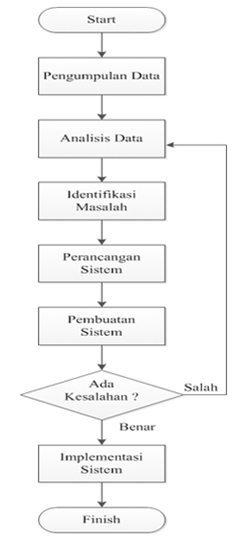
\includegraphics[width=0.5\textwidth]{gambar/flow}
    \caption{Flowchart Metode Penelitian}

\end{figure}

Keterangan Flowchart :
\begin{itemize}
\item[1.] Pada penelitian  ini penulis memulai penelitian dengan mengumpulkan data dari sumber yang terlibat langsung dalam penelitian.Pengumpulan data di ambil langsung dari metode observasi dimana metode pengumpulan data dengan mengamati langsung kegiatan-kegiatan  yang dilakukan di Dinas Pariwisata. Selain itu juga menggunakan metode wawancara ,di mana dengan metode ini untuk mendapatkan data-data yang dibutuhkan dengan pihak-pihak yang berkepentingan di Dinas Pariwisata. 
\item[2.] Setelah data dari sumber cukup, maka akan dilakukan analisis data yaitu menganalisis  kebutuhan  sistem  dari hasil pengambilan data yang telah di lakukan dengan metode observasi dan wawancara. 
\item[3.]Setelah semua data terkumpul langkah selanjutnya yaitu mengidentifikasi masalah dan mengevaluasi  permasalahan  kebutuhan sistem yang terdapat dalam sistem yang lama  sehingga dapat diusulkan perbaikannya untuk membuat suatu sistem yang baru.
\item[4.]Kemudian di lakukan tahap perancangan sistem baru dimana Sistem baru yang akan di buat, perancangan sistemnya  berdasarkan  analisis  dan identifikasi masalah yang  telah dilakukan.
\item[5.]Setelah tahap perancangan sistem selesai maka akan dilakukan pembuatan sistem baru yaitu untuk  menterjemahkan  perancangan sistem  ke  dalam  bahasa  pemrograman  yang  telah ditentukan, yang akan di gunakan sebagai pemecahan masalah pada Dinas Pariwisata Kabupaten Jember.
\item[6.]Bila pada sistem yang telah ada masih mengalami kesalahan  ataupun kekurangan maka  proses akan di lakukan kembali dari tahap analisis data, dan apabila sistem tersebut sudah memenuhi, maka akan di lanjutkan ke tahapan berikutnya.
\item[7.]Tahapan selanjutnya yaitu implementasi sistem dimana mengimplementasikan  hasil  pembuatan sistem  menjadi  sebuah  sistem informasi dan dapat di gunakan langsung pada Dinas Pariwisata di Jember.
\end{itemize}

\section{Tehnik Pengumpulan Data}
Untuk dapat melaksankan tahapan penelitian maka tahapan penelitian yang dilakukan adalah sebagai berikut: 
\subsection{Studi Pustaka} 
Studi pustaka merupakan langkah awal dalam metode pengumpulan data. Studi pustaka merupakan metode pengumpulan data yang diarahkan kepada pencarian data dan informasi melalui dokumen-dokumen, baik dokumen tertulis, foto-foto, gambar, maupun dokumen elektronik yang dapat mendukung dalam proses penulisan.”Hasil penelitian juga akan semakin kredibel apabila didukung foto-foto atau karya tulis akademik dan seni yang telah ada.”(Sugiyono,2005:83). Studi pustaka merupakan Maka dapat dikatakan bahwa studi pustaka dapat memengaruhi kredibilitas hasil penelitian yang dilakukan. 
\subsection{Metode Pengumpulan data}  
Pengumpulan data dilakukan untuk memperoleh informasi yang dibutuhkan dalam rangka mencapai tujuan penelitian. Tujuan yang diungkapkan dalam bentuk hipotesis merupakan jawaban sementara terhadap pertanyaan penelitian.metode pengumpulan data bisa dilakukan dengan cara:
\begin{itemize}
\item[a.] Data Primer primer diperoleh melalui:
\begin{itemize}
\item[1.] Observasi
Merupakan metode pengumpulan data dengan mengamati langsung kegiatan-kegiatan  yang dilakukan pada Dinas Pariwisata Jember mulai  dari  pengelolaan data objek wisata, hotel, dan kuliner
\item[2.]Wawancara 
 Melakukan wawancara untuk mendapatkan data-data yang di butuhkan dengan pihak-pihak yang berkepentingan di Dinas pariwisata untuk mengetahui alur pengelolaan data objek wisata.
\end{itemize}
\item[b.]Data sekunder diperoleh melalui:
\begin{itemize}
\item[1.]Studi dokumentasi
Studi dokumentasi dalam penelitian ini yaitu menggunakan data yang sudah ada yang di peroleh dari Dinas Pariwisata.
\item[2.]Akses internet
Akses internet digunakan untuk mencari data pendukung dari berbagai buku,ebook,maupun jurnal-jurnal yang relevan.
\end{itemize}
\end{itemize}



\section{Jadwal Kegiatan}
Penelitian direncanakan akan dilaksanakan selama enam bulan. Rincian rencana jadwal penelitian dicantumkan dalam tabel berikut.

\begin{center}
Tabel 3.1. Jadwal Penelitian.
\end{center}
\vspace{-0.5cm}
\begin{figure}[ht!]
  \centering
    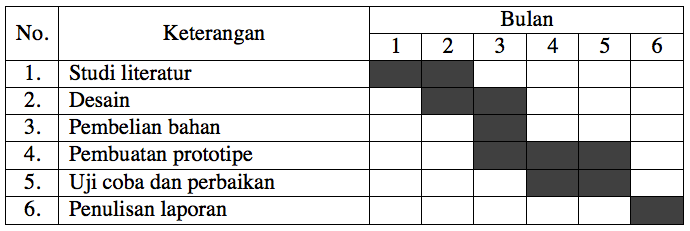
\includegraphics[width=13cm]{gambar/timeline}
\end{figure}

%-----------------------------------------------------------------
%Disini akhir masukan Bab
%-----------------------------------------------------------------

%-----------------------------------------------------------------
%Disini awal masukan untuk Daftar Pustaka
%-----------------------------------------------------------------
%%\nocite{Abel2010,Guerbas201350}
%%\bibliography{research-plan}
%%\bibliographystyle{plainnat}
\begin{thebibliography}{9}

\bibitem[satu(2011)]{satu01}
Safaat, Nazarudin. 2011. Pemrograman Aplikasi Mobile Smartphone dan Tablet PC Berbasis Android, Bandung: Informatika.

\bibitem[dua(2010)]{dua02}
Johanes, 2010. JAVA ME Membangun Berbagai Aplikasi Handphone.Jakarta : Jasakom 

\bibitem[tiga(2001)]{tiga03}
Dharwiyanti, Romi S.W. 2003. Pengantar Unified Modelling Language (UML).

\bibitem[empat(2012)]{empat04}
Irawan. 2012. Membuat aplikasi Android Untuk Orang Awam.Palembang:Maxiko

\bibitem[lima(2013)]{lima05}
No Name.  Jember Tourism. Diakses 10-10-2014 Url :http://jembertourism.com/

\bibitem[enam(2013)]{enam06}
No Name. Use Case. Diakses 10-10-2014 Url : http: //omhegar.blogspot.com/ 2013/08/pengertian-use-case-dan-contoh-use-case.html


\end{thebibliography}
\addcontentsline{toc}{chapter}{DAFTAR PUSTAKA}
%-----------------------------------------------------------------
%Disini akhir masukan Daftar Pustaka
%-----------------------------------------------------------------

\end{document}